%!TEX root=main.tex
\chapter{Evaluation}
\label{cha:evaluation}

\chapterquote{An ounce of performance is worth pounds of promises.}{Mae West, (1893 - 1980)}

In this chapter we will investigate the scalability of Gilbert and how it performs compared to famous hand-tuned ML algorithms.
We hope to show that Gilbert is not only easily usable in terms of programming but also produces results with decent performance.
Furthermore, we want to compare the different execution engines and math-backends to see which system gives the best results.
Based on these outcomes, we want to come up with a recommendation for the best settings of Gilbert.

For our evaluation, we used the $400$-core cluster provided by the DIMA faculty of the Technical University of Berlin.
The cluster comprises $25$ local machines with each \SI{32}{\giga\byte} of main memory.
Each machine is equipped with $2$ AMD Opterons 6128 CPUs, each of them having $8$ cores.
The CPUs run at a speed of \SI{2}{\giga\hertz}.

We employ Apache Spark-1.0.0~\cite{spark} for our test runs with the Spark execution engine.
For the Stratosphere execution engine, we use a slightly extended version of Stratosphere-0.6-SNAPSHOT~\cite{stratosphere}.
At the time of writing this thesis, Stratosphere-0.6 was still under development but we needed the latest features.
Therefore, we used the current snapshot version.
All extensions made to the current snapshot version are also pending pull requests and we hope that the final release will contain them all.
Thus, executing Gilbert with the stable relase Stratosphere-0.6 should work fine.
As the underlying distributed filesystem both systems use Apache Hadoop-1.2.1~\cite{hadoop:2008a}.

\section{Scalability}

The scalability evaluation investigates how Gilbert behaves under increasing work loads and how well it can exploit varying cluster sizes.
As we have implemented Gilbert with the intention to provide a scalable linear algebra environment, it is important that it can process data sizes exceeding the main memory of a single machine.
We want to evaluate the scalability performance for the Stratosphere and Spark execution engine.

\subsection{Matrix Multiplication}
\label{subsec:mm}

As a first benchmark, we have chosen the matrix multiplication $A\times B$ with $A,B \in \mathbb{R}^{n\times n}$ and $n$ being the dimensionality.
The matrix multiplication operation is demanding both in CPU load as well as network I/O.
The implementation of the matrix multiplication, shown in \cref{sec:LinearAlgebraOperations}, first joins the column blocks of the left matrix with the row blocks of the right matrix.
This operation replicates the two operands partially and sends them across the network to their respective worker nodes.
Afterwards, for each matching pair of blocks a local matrix multiplication is executed, which has a complexity of $\mathcal{O}(n_{block}^3)$ with $n_{block}$ being the block size.
The produced intermediate results are grouped according to their left row index and right column index.
Finally, the grouped result blocks are added up to !! the final result.

The matrices $A$ and $B$ are sparse matrices with uniformly distributed non-zero cells.
They are randomly generated prior to the matrix mutliplication, thereby avoiding costly file system I/O.
The sparsity of both matrices is set to $0.001$.
Therefore, both matrices are represented by sparse matrix implementations.
As a baseline, we run the same matrix multiplication on a single machine of the cluster using Gilbert's local execution engine.
The local execution engine uses the same math-backend as the distributed engines and thus serves as a good reference value to see the additional costs of parallel execution.
Breeze was chosen as the math back end for the matrix multiplication.
The Stratosphere and Spark execution engines are both started with \SI{20}{\giga\byte} of main memory for their task managers.
Furthermore, they are both configured to use a similar scheduling strategy, which distributes the work equally among the available computer nodes.
This is especially important in order to compare the results, because some parts of Breeze are multi-threaded and consequently takes advantage of idling cores.

In the first experiment, we fixed the block sizes to $500 \times 500$ and set the number of cores to $50$.
We then increased the dimensionality $n$ of $A$ and $B$ to observe the runtime behavior.
The resulting execution times for the local, Stratosphere and Spark execution engines are shown in \cref{fig:mmLoadRuntime}.

\begin{figure}
	\centering
	\begin{subfigure}{\dualpgfwidth}
		\begin{tikzpicture}
			\begin{loglogaxis}[
				xlabel={Dimensionality $n$},
				ylabel={Execution time $t$ in s},
				width=\dualpgfwidth,
				legend entries={Local, Spark, Stratosphere},
				legend pos=north west,
			]
			\addplot[
				color=blue,
				mark=x,
			] table[
				x=RowsA,
				y=Time,
			]
			{data/matrixMultLoad/matrixMultLoadReference};
			\addplot[
				color=red,
				mark=o,
			] table[
				x=RowsA,
				y=Time,
			]
			{data/matrixMultLoad/matrixMultLoadSpark};
			\addplot[
				color=teal,
				mark=triangle,
			] table[
				x=RowsA,
				y=Time,
			]
			{data/matrixMultLoad/matrixMultLoadStratosphere};
			\end{loglogaxis}
		\end{tikzpicture}
		\caption{}
		\label{fig:mmLoadRuntime}
	\end{subfigure}
	\begin{subfigure}{\dualpgfwidth}
		\begin{tikzpicture}
			\begin{semilogxaxis}[
				xlabel={\#cores},
				ylabel={Execution time $t$ in s},
				width=\dualpgfwidth,
				legend pos=north west,
				legend entries={Spark, Stratosphere},
				ymin=0.0,
				ymax=275,
			]
			\addplot[
				color=red,
				mark=o,
			] table[
				x=Parallelism,
				y=Time,
			]
			{data/matrixMultCores/matrixMultCoresSpark};
			\addplot[
				color=teal,
				mark=triangle,
			] table[
				x=Parallelism,
				y=Time,
			]
			{data/matrixMultCores/matrixMultCoresStratosphere};
			\end{semilogxaxis}
		\end{tikzpicture}
		\caption{}
		\label{fig:mmNodesRuntime}
	\end{subfigure}
	\caption{Scalability of matrix multiplication. \subref{fig:mmLoadRuntime} Execution time of matrix multiplication depending on the data size on a $50$-core cluster. \subref{fig:mmNodesRuntime} Execution time of matrix multiplication depending on the cluster size with constant per core work load.}
	\label{fig:mmBenchmark}
\end{figure}

On a single machine, we could execute the matrix multiplication for dimensionalities up to $n=10000$ before the system ran out of memory.
We can see that the local execution performs better for dimensionalities $n \le 5000$.
That was expected since the matrix still fits completely in the main memory of a single machine and the distributed execution adds some significant communication overhead.
Futhermore, Spark and Stratosphere both exhibit some noticeable job start up latency which is dominating the execution time for $n\le 10000$.
Those are the reasons why the local executor performs better than the distributed implementations for small matrix sizes.

For matrices with $n>5000$, Spark starts to calculate the matrix multiplication faster than the local executor.
The Stratosphere execution engine does not beat the local computation for sizes which are manageable by a single machine, though.
However, we can observe a steeper ascent of the local execution time compared to Stratosphere.

We also see that Gilbert can handle matrix sizes which scale far beyond the memory capacity of a single machine.
The matrix multiplication for $n=64000$ was finished in \SI{719}{\second} on Spark and in \SI{1230}{\second} on Stratosphere.
We can observe that the Spark execution engine runs continuously faster than Stratosphere.
Since the work load is similar for both systems, the difference has to be caused by the internal functioning of both systems.
For smaller dimensionalities, the execution time of both systems stays almost the same.
Therefore, it has to be mainly caused by the job start up times.
We can consequently infer that the start up times of Spark are lower than those of Stratosphere.
For $n>10000$, the speed up of Spark compared to Stratosphere is roughly $2$.

In the second experiment, we investigate the scaling behavior of Gilbert with respect to the cluster size.
As a benchmark, we calculate again $A\times B$ with $A,B \in \mathbb{R}^{n\times n}$ and $n$ being the dimensionality.
In order to observe the inflicted communication costs, we keep the per core work load constant while increasing the number of cores.
For this experiment we varied the number of cores from $1$ to $100$ and scaled $n$ such that $n^3/\#\text{cores}$ is constant.
We started with $n=7500$ for a single core and reached $n=35000$ on $100$ cores.
As blocksize we chose $500\times 500$.
The results of the experiment are shown in \cref{fig:mmNodesRuntime}.

The optimal scale-out behavior would be a horizontal line.
However, it is impossible to achieve this scale-out behavior due to several reasons, such as network communications and synchronization.
Nonetheless, the results depicted in \cref{fig:mmNodesRuntime} indicate for both execution engines decent scale-out behavior.
Especially for the number of cores $\le 15$, we observe for Stratosphere and Spark an almost horizontal line.
From this point onwards, the scaling of Stratosphere degrades faster than Spark's scaling.
Spark exhibits an almost perfect scale-out behavior.
The time it requires to calculate a matrix multiplication with $n=7500$ on a single core is almost identical to the \SI{90}{\second} it needs to calculate the matrix multiplication with $n=35000$ on $100$ cores.
Interestingly, Spark's graph is not monotonic, as one would expect it.
For $\text{\#cores}=50$, we can observe a slight peek in execution time.
This behavior is counterintuitive it has to be linked to the internal functioning of the Spark system.

\subsection{Non-negative Matrix Factorization}
\label{subsec:NMF}

As second benchmark for evaluating the scalability properties, we have chosen the non-negative matrix factorization (NMF) algorithm~\cite{seung:anips2001a}.
NMF finds for a given matrix $V$ a factorization $W$ and $H$ such that $V\approx W H$ holds.
The algorithm is a popular ML algorithm which finds application in computer vision, document clustering and topic modeling.
In the context of topic modeling, we would have $d$ documents and a set of $w$ words which are contained in the documents.
The goal of topic modeling is to identify the different topics and the words supporting a particular topic.
For this purpose, the matrix $V = (v_{i,j})_{i=1\ldots d,j=1\ldots w}$ is defined, with $v_{i,j}$ containing the frequency of a word $w_j$ appearing in document $d_i$.
By specifying the number of topics $t$, the NMF algorithm computes $W\in \mathbb{R}^{d\times t}$ and $H\in \mathbb{R}^{t\times w}$ such that $V \approx W H$.
The row $w_i$ of $W$ indicates which topics the document $d_i$ contains and the row $h_i$ of $H$ tells us which words correlate with topic $t_i$.
The NMF algorithm alternately updates the matrices $H$ and $W$ until the result converges.
The algorithm is given in \cref{lst:nmf}.
The operator $.*$, $./$ and $*$ denote the cell wise multiplication, the cell wise division and the matrix multiplication, respectively.

\begin{listing}[!h]
	\begin{CenteredBox}
		\begin{lstlisting}[language=Matlab]
		V = load(); % load matrix to factorize
		W = load(); % load initial values of W
		H = load(); % load initial value of H

		while i < maxIterations
			H = H.*(W'*V ./ W'*W*H); % udpate H
			W = W.*(V*H' ./ W*H*H'); % update W
			i = i + 1;
		end
		\end{lstlisting}
	\end{CenteredBox}
	\caption{Non-negative matrix factorization algorithm.}
	\label{lst:nmf}
\end{listing}

We have chosen NMF, because it represents an actual ML algorithm which had recently been implemented for MapReduce systems~\cite{liu:2010a}.
As far as we know, the proposed MapReduce algorithm is one of the best distributed implementations of NMF.
Thus, it is well suited to assess the performance of Gilbert's implementation of NMF.

For our evaluation we calculate one step of the NMF algorithm.
We set $t=10$, $w=100000$ and vary the number of documents $d$.
The matrix $V\in\mathbb{R}^{d\times 100000}$ is a sparse matrix whose sparsity is set to $0.001$.
The non-zero cells of $V$ are uniformly distributed.
Thus, each line of $V$ contains roughly $100$ non-zero entries, which are drawn from a Gaussian distribution.
The matrices $W$ and $H$ are dense and initialized with random values drawn from a Gaussian distribution as well.
As a baseline, we run the NMF on a single machine of the cluster using the local execution engine.
As math back end we chose the Breeze library, which is also used for the distributed execution engines.
Like for the matrix multiplication benchmark, the task manager of Spark and Stratosphere are started with \SI{20}{\giga\byte} of memory and both systems use the same scheduling strategy keeping the work load on all nodes equally distributed.

In the first experiment we fixed the number of cores to $50$ and investigated the runtime behavior for increasing values of $d$.
We started with $d=500$ and increased the number of rows of $V$ to $150000$.
The block size for Gilbert was set to $500 \times 500$.
In order to fairly compare the results with the optimized NMF MapReduce implementation proposed in~\cite{liu:2010a}, we reimplemented the algorithm using the Spark and Stratosphere runtime system.
This hand-tuned implementation, henceforth denoted as GNMF, was also executed on $50$ cores.
Additionally, the data was generated having the respective partitioning required by the algorithm.
The execution times of GNMF and Gilbert's NMF are shown in \cref{fig:nmfLoadRuntime}.

\begin{figure}
	\centering
	\begin{subfigure}{\dualpgfwidth}
		\begin{tikzpicture}
			\begin{loglogaxis}[
				xlabel={Rows $d$ of $V$},
				ylabel={Execution time $t$ in s},
				width=\dualpgfwidth,
				legend pos=north west,
				legend entries={Local, Spark, Stratosphere, GNMF Spark, GNMF Stratosphere},
				ymax=5000,
			]
			\addplot[
				color=blue,
				mark=x,
			] table[
				x=Rows,
				y=Time,
			]
			{data/nnmfStepLoad/nnmfStepLoadReference};
			
			\addplot[
				color=red,
				mark=o,
			] table[
				x=Rows,
				y=Time,
			]
			{data/nnmfStepLoad/nnmfStepLoadSpark};
			
			\addplot[
				color=teal,
				mark=triangle,
			]table[
				x=Rows,
				y=Time,
			]
			{data/nnmfStepLoad/nnmfStepLoadStratosphere};
			\addplot[
				color=black,
				mark=diamond,
			]table[
				x=rowsV,
				y=time,
			]
			{data/nnmfStepLoad/gnmfStepLoadSpark};
			\addplot[
				color=magenta,
				mark=square,
			]table[
				x=rowsV,
				y=time,
			]
			{data/nnmfStepLoad/gnmfLoadStratosphere};
			\end{loglogaxis}
		\end{tikzpicture}
		\caption{}
		\label{fig:nmfLoadRuntime}
	\end{subfigure}
	\begin{subfigure}{\dualpgfwidth}
		\begin{tikzpicture}
			\begin{semilogxaxis}[
				xlabel={$\#cores$},
				ylabel={Execution time $t$ in s},
				width=\dualpgfwidth,
				ymin=0,
				legend entries={Spark, Stratosphere},
				legend pos=north west,
			]
			\addplot[
				color=red,
				mark=o,
			] table[
				x=Parallelism,
				y=Time,
			]
			{data/nnmfStepCores/nnmfStepCoresSpark};

			\addplot[
				color=teal,
				mark=diamond,
			] table[
				x=Parallelism,
				y=Time,
			]
			{data/nnmfStepCores/nnmfStepCoresStratosphere};
			\end{semilogxaxis}
		\end{tikzpicture}
		\caption{}
		\label{fig:nmfNodesRuntime}
	\end{subfigure}
	\caption{Scalability of NMF. \subref{fig:nmfLoadRuntime} Execution time of one NMF step depending on the data size on a $50$-core cluster. \subref{fig:nmfNodesRuntime} Execution time of one NMF step depending on the cluster size with constant per core work load.}
	\label{fig:nmfBenchmark}
\end{figure}

The local executor could be applied to sizes of $d$ ranging from $500$ to $1500$ rows, before the data exceeded the available main memory of a single computer.
As expected, the local execution performs far better for these data sizes than the distributed execution with Stratosphere.
However, the Gilbert NMF and the GNMF executed on Spark outperformed the local execution.
That is rather surprisingly, since the distributed execution should inflict some noticeable communication overhead.
But apparently, the parallelism compensates for the additional communication costs.

The distributed systems can also be used for data sizes which exceed the memory of a single computer.
Both distributed execution engines scale well up to the point where Spark and Stratosphere can no longer keep the data in memory.
The two data flow systems have to perform internal sorting, partitioning and shuffling steps to implement the high level operations, such as join, reduce, cogroup and cross.
If the memory size is not sufficient to execute these steps, then the data will be gracefully spilled to disk.
On the one hand, this behavior makes the systems more robust and applicable to data sizes which largely exceed the total amount of memory.
But on the other hand, the performance abruptly deteriorates massively once the data has to be spilled.
For the Stratosphere and Spark executor, we experienced this behavior for $d>50000$ and $d>150000$, respectively.
For data sizes bigger than these thresholds, the benchmark runs became so slow that we could not finish them and discarded these runs as infeasible.

For Stratosphere, this behavior ensues earlier due to its specific memory management.
Stratosphere assigns each cluster node a specific number of slots.
The default value is the number of cores.
The memory is then split evenly among the slots.
Once the task managers have started and assigned the memory to each slot, it is not possible to dynamically transfer memory portions between slots.
Therefore, the effectively available memory for each task is considerably smaller than the initial \SI{20}{\giga\byte}.
Additionally, Stratosphere's ability to support streaming further decreases the per task memory.
Currently, it is assumed that all tasks belonging to one pipeline can be deployed simultaneously to one slot.
In order to execute all pipeline tasks, the slot memory will be further divided by the number of tasks which can be concurrently run.

In contrast to that, Spark separates the execution of different operations into distinct stages.
A stage is only submitted for execution, after all preceding stages have been completed.
That way, the memory does not have to be splitted between succeeding tasks and thus spilling occurs later.

The runtime between the optimized GNMF running on Spark, the Stratosphere and the Spark executor differed for varying data sizes by a constant factor.
The fastest implementation for $d\le 100000$ was the optimized GNMF algorithm running on Spark.
It was approximately twice as fast as Gilbert's Spark execution engine.
The Stratosphere execution engine was approximately five times slower than its Spark counterpart.
These differences are most likely caused by the Spark and Stratosphere system, since the linear algebra operations are implemented identically.
The runtime behavior of the optimized GNMF running on Stratosphere is interesting.
At first, it performs rather poorly compared to its Spark counterpart.
However, for $d>100000$ it suddenly outperforms the Spark implementation.
Thus, GNMF scales better if it is executed on Stratosphere. 

Even though, Gilbert could not reach or even beat the performance of the optimized GNMF implementation, the development using Gilbert was considerably easier.
One NMF step can be programmed in two lines of Gilbert code, whereas we needed $35$ lines of Scala code for GNMF.
Not only did we have to know how to program Spark, but it also took us quite some time to verify the correct functioning of the Spark implementation.
The verification was made significantly more difficult and time-consuming due to a programming bug we introduced.
The debugging process showed us quite plainly how tedious the development process even with systems like Spark and Stratosphere can be.
Thus, the productivity increase gained by using a high-level declarative programming language for linear algebra must not be neglected and compensate for the performance loss.
\Textcite{alvaro:2010a} made a similar observations when developing a declarative programming language for distributed systems programming.

In the second experiment of the NMF benchmark, we analyze how Gilbert scales-out when increasing the cluster size while keeping the work load for each core constant.
We vary the cluster size from $1$ core to $100$ cores and scale the number of documents $d$ accordingly.
Initially we start with $1000$ documents and, consequently, calculate the matrix factorization for $100000$ documents on $100$ cores.
The ideal behavior would be a horizontal line.
However, this cannot be expected, since the NMF computation requires communication between the cluster nodes.
The results of this experiment are shown in \cref{fig:nmfNodesRuntime}.

The scale-out behavior of the Stratosphere and Spark execution engine both show a good result for $\#cores \le 5$.
For higher degree of parallelism, Stratosphere's performance quickly deteriorates.
On $50$ cores, Stratosphere needs \SI{1082}{\second}, whereas Spark needs only \SI{113}{\second}.
We could not finish Stratosphere's computations for higher degrees of parallelism than $50$, because the system simply became too slow.
That vast performance decline is most likely caused by data spilling at some internal operation.
In contrast to Stratosphere, Spark does not suffer from these limitations for the number of cores we tested.
In fact, it almost exhibits a perfect scale-out behavior with a constant runtime.
The runtime on $100$ cores is only two times slower than the runtime on a single core with the same work load per core.

\subsection{Block Size}

The block size has a significant influence on the overall performance of Gilbert since it directly controls the data parallelism and data granularity of the local operations.
The bigger the block size is, the fewer blocks are available for parallel computation.
But the bigger the block size is, the more work can be done on a single computer without having to communicate with other nodes.
To measure the effect of the block size on the performance, we calculate one NMF step with varying block sizes using the Spark execution engine.
For this benchmark we set $d=100000$, $w = 100000$ and $t = 10$.
The execution times for different block sizes are shown in \cref{fig:blocksizesNMFStep}.

\begin{figure}
	\centering
	\begin{subfigure}[t]{\dualpgfwidth}
		\begin{tikzpicture}
			\begin{axis}[
				ymin=0,
				ylabel={Execution time $t$ in s},
				width=\dualpgfwidth,
				ybar,
				xtick={0,1,2,3,4,5},
				xticklabels={
				25 x 25,
				50 x 50,
				100 x 100,
				500 x 500,
				1000 x 1000,
				2000 x 2000
				},
				x tick label style={rotate=45,anchor=east, /pgf/number format/1000 sep=},
				height=159pt,
			]
			\addplot[
				color=blue,
				fill=blue,
			]table[
				x=Idx,
				y=Time,
			]
			{data/nnmfStepBlocksizes/nnmfStepBlocksizesSpark100000};
			\end{axis}
		\end{tikzpicture}
		\caption{}
		\label{fig:blocksizesNMFStep}
	\end{subfigure}
	\begin{subfigure}[t]{\dualpgfwidth}
		\begin{tikzpicture}
			\begin{loglogaxis}[
				xlabel={Rows $d$ of $V$},
				ylabel={Execution time $t$ in s},
				width=\dualpgfwidth,
				legend entries = {25 x 25, 500 x 500, 1000 x 1000},
				legend pos=north west,
			]
			\addplot[blue,
				mark=x,
			] table[
				x=Rows,
				y=Time,
			]
			{data/nnmfStepBlocksize/nnmfStepBlocksize25Spark};

			\addplot[red,
				mark=o,
			] table[
				x=Rows,
				y=Time,
			]
			{data/nnmfStepBlocksize/nnmfStepBlocksize500Spark};

			\addplot[teal,
				mark=diamond,
			] table[
				x=Rows,
				y=Time,
			]
			{data/nnmfStepBlocksize/nnmfStepBlocksize1000Spark};
			\end{loglogaxis}
		\end{tikzpicture}
		\caption{}
		\label{fig:nmfStepDifferentBlocksizes}
	\end{subfigure}
	\caption{Execution time for different block sizes. \subref{fig:blocksizesNMFStep} Execution time of one NMF step with constant input depending on the block size on a $50$-core cluster using the Spark execution engine. \subref{fig:nmfStepDifferentBlocksizes} Execution time of one NMF step depending on the number of rows for different block sizes on a $50$-core cluster using the Spark execution engine.}
	\label{fig:blocksizes}
\end{figure}

The graph shows that we have a minimal runtime for a block size of $500 \times 500$.
Apparently, this block size constitutes the best trade-off between data parallelism and data granularity.
For lower block sizes, the additional overhead introduced by indexing information and the low data granularity increases the runtimes.
For higher block sizes, the decreased parallelism devours the benefits of a high data granularity.
That evaluation justifies our block size choice of $500 \times 500$.

The effect of different block sizes is also compared in \cref{fig:nmfStepDifferentBlocksizes} where we computed one NMF step with the Spark execution engine for varying sizes of $V$.
The NMF algorithm is executed on $50$ cores of the cluster using the Breeze math back end.
We can observe that we obtain better results with an increased block size.
Clearly, the block size $25 \times 25$ is inferior to the block sizes $500\times 500$ and $1000\times 1000$.
However, the results between the last two block sizes do not differ significantly.

\subsection{Optimization}

In this subsection, we want to evaluate the effects Gilbert's optimizer has on the runtime of programs.
For this purpose, we execute one NMF step on Gilbert's Stratosphere and Spark execution engine using the same settings as in \cref{subsec:NMF}.
However, this time we disable the transpose pushdown and matrix-multiplication reordering optimization.
The results are shown in \cref{fig:nnmfLoadOptimization}.

\begin{figure}
	\centering
	\begin{tikzpicture}
		\begin{semilogxaxis}[
			xlabel={Rows $d$ of $V$},
			ylabel={Execution time $t$ in s},
			legend pos=north west,
			legend entries={Optimized Spark, Optimized Stratosphere, Non-optimized Spark, Non-optimized Stratosphere},
		]
		
		\addplot[
			color=red,
			mark=o,
		] table[
			x=Rows,
			y=Time,
		]
		{data/nnmfStepLoadNoOp/nnmfStepLoadSpark};
		
		\addplot[
			color=teal,
			mark=triangle,
		]table[
			x=Rows,
			y=Time,
		]
		{data/nnmfStepLoadNoOp/nnmfStepLoadStratosphere};

		\addplot[
			color=blue,
			mark=x,
		] table[
			x=Rows,
			y=Time,
		]
		{data/nnmfStepLoadNoOp/nnmfStepNoOpLoadSpark};

		\addplot[
			color=black,
			mark=diamond,
		]table[
			x=Rows,
			y=Time,
		]
		{data/nnmfStepLoadNoOp/nnmfStepNoOpLoadStratosphere};
		
		\end{semilogxaxis}
	\end{tikzpicture}
	\caption{Runtime of Gilbert's optimized and non-optimized single nnmf step on $50$-core cluster.}
	\label{fig:nnmfLoadOptimization}
\end{figure}

We can observe that Gilbert's optimizer has a significant effect on the runtime of NMF.
The optimized Gilbert program runs on both distributed engines faster than it's non-optimized counterpart.
Interestingly, the Spark execution engine seems to benefit more from the optimizer than the Stratosphere executor.
For $d=10000$, the optimized Spark version runs about $18$ times faster than the non-optimized program.
Stratosphere shows only a speed-up of roughly $1.7$ between the optimized and non-optimized version.

It is not yet known what causes these different speed-ups.
However, looking at the NMF formula in \cref{lst:nmf}, we can explain why the optimization works.
There are two matrix multiplications which can be optimized: $W^\prime WH$ in line $6$ and $WHH^\prime$ in line $7$.
Keeping in mind that $W\in \mathbb{R}^{d\times 10}$ and $H\in \mathbb{R}^{10 \times 100000}$, we can assess the different strategies.
The non-optimized version would execute the matrix multiplications due to left-associativity from left to right:

\begin{displaymath}
	\overbrace{\underbrace{\left(W^\prime W\right)}_{\in \mathbb{R}^{10\times 10}}H}^{\in\mathbb{R}^{10\times 100000}}
\end{displaymath}

and

\begin{displaymath}
	\overbrace{\underbrace{\left(WH\right)}_{\in \mathbb{R}^{d \times 100000}}H^\prime}^{\in \mathbb{R}^{d\times 10}}
\end{displaymath}

For the first matrix multiplication, the execution order is optimal, since the intermediate result of $W^\prime W$ is much smaller than $WH$.
However, for the second matrix multiplication, the execution order is far from optimal.
The left-associativity produces an intermediate matrix result of size $d\times 100000$.
For large $d$ this matrix becomes really huge.
Additionally, the intermediate result is dense, because the operands $W$ and $H$ are dense as well.
By changing the execution order, we can decrease the size of the intermediate result significantly.

\begin{displaymath}
	\overbrace{W\underbrace{\left(HH^\prime\right)}_{\in \mathbb{R}^{10 \times 10}}}^{\in \mathbb{R}^{d\times 10}}
\end{displaymath}

Gilbert's optimizer first detects the matrix multiplication reordering and then changes it so that the maximum intermediate result is minimized.
That is the reason why the optimized NMF program runs clearly faster.

\section{Gilbert Algorithms vs. Specialized Algorithms}

In this section, we want to investigate how well algorithms implemented in Gilbert perform compared to specialized algorithms.
We expect that the Gilbert runtime adds some overhead as trade-off for their easy to use programming interface.
Furthermore, the high-level linear algebra abstraction of Gilbert might make it diffcult to exploit certain properties to speed up the processing.
Therefore, we believe that hand-tuned algorithms will get the upper hand.

For our comparison, we have chosen two famous ML algorithms which can be expressed in terms of linear algebra: PageRank and k-means.
Since both algorithms are iterative, we can demonstrate Gilbert's loop support.
We first execute them directly in Gilbert, given the Matlab code, and then run them directly on Stratosphere and Spark.
For the direct execution, we have implemented both algorithms using the Stratosphere and Spark API.
In contrast to Gilbert, the direct implementation required a deep understanding of the underlying runtime system.
Furthermore, the distributed implementation was far from trivial compared to the linear algebra representation of the original problem.

\subsection{PageRank}

The PageRank algorithm~\cite{page:1999a} is the famous algorithm developed by Larry Page and Sergey Brin to compute a ranking between any kind of entities with reciprocal quotations and references.
Initially, it was developed to rank the websites of the world wide web, which it does so well that Google grew quickly into a multi-billion dollar company.
However, PageRank is only one algorithm comprising Google's web search, but probably the best known.

The idea of PageRank is to estimate the rank of a web site based on the ranks of the websites, which link to this site.
It is assumed that high quality web sites are more likely to link to other high quality web sites.
Thus, these sites get a high rank with which they can "vote" for other sites.

The PageRank can also be explained by the model of a "random" surfer.
Assume there is a surfer which randomly follows an outgoing link from a web site.
Occasionally, or if he ends up in a dead end, the surfer enters a random url in his address bar.
That way, he will eventually visit the whole web.
By tracking the time he spends on each web site, we get an importance measure for each site.
Pages, which are linked by pages on which the random surfer spends more time, will receive more clicks by the random surfer and thus a higher importance.
That importance measure is in fact the PageRank.

\begin{listing}[!h]
	\begin{CenteredBox}
		\begin{lstlisting}[language=Matlab]
		% load adjacency matrix
		A = load(); 
		maxIterations = 10;
		d = sum(A, 2); % outdegree per vertex
		% create the column-stochastic transition matrix
		T = (diag(1 ./ d) * A)'; 
		r = ones(numVertices, 1) / numVertices; % initialize the ranks
		e = ones(numVertices, 1) / numVertices;
		% PageRank calculation
		while i < maxIterations
			r = .85 * T * r + .15 * e
			i = i + 1
		end
		\end{lstlisting}
	\end{CenteredBox}
	\caption{Matlab's PageRank implementation.}
	\label{lst:PageRankVanilla}
\end{listing}

Even though the problem seems to be self-referencing, the PageRank vector turns out to be the solution to an eigenvalue problem.
Thus, the PageRank vector can easily be computed using a power iteration.
PageRank's Matlab code is given in \cref{lst:PageRankVanilla}.

The power iteration happens in the while loop, where we iteratively multiply the PageRank vector $r$ with the transition matrix $T$.
In order to execute this code with Gilbert, we only have to replace the while loop with a fixpoint operation.
As it can be seen in \cref{lst:gilbertPageRank}, the replacement is only of syntactic nature.

\begin{listing}[!h]
	\begin{CenteredBox}
		\begin{lstlisting}[language=Matlab]
		% load adjacency matrix
		A = load();
		maxIterations = 10;
		d = sum(A, 2); % outdegree per vertex
		% create the column-stochastic transition matrix
		T = (diag(1 ./ d) * A)'; 
		r_0 = ones(numVertices, 1) / numVertices; % initialize the ranks
		e = ones(numVertices, 1) / numVertices;
		% PageRank calculation
		fixpoint(r_0, @(r) .85 * T * r + .15 * e, maxIterations)
		\end{lstlisting}
	\end{CenteredBox}
	\caption{Gilbert's PageRank implementation.}
	\label{lst:gilbertPageRank}
\end{listing}

An usual direct implementation of PageRank for Spark and Stratosphere works as follows.
The PageRank vector is represented by a set of tuples $(w_i, r_i)$ with $w_i$ denoting the web site $i$ and $r_i$ being its rank.
The adjacency matrix is stored row-wise as a set of tuples $(w_i, a_i)$ with $w_i$ denoting the web site $i$ and $a_i$ being the adjacency list of web site $i$.
For the adjacency list $a_i$ it holds that $w_j \in a_i$ if and only if there exists a link from web site $i$ to $j$.

Given the PageRank vector and the adjacency matrix representation, we can compute the next PageRank vector the following way.
At first, the PageRank $r_i$ of web site $i$ is joined with its adjacency list $a_i$.
For each outgoing link $w_j \in a_i$ we create a new tuple $(w_j, 0.85r_i/\left|a_i\right|)$ with the rank of $i$ being divided by the number of outgoing links.
In order to incroporate the random jump behavior to any available web site, a tuple $(w_i, 0.15/|w|)$, with $|w|$ being the number of all websites, is generated for each website $i$.
In order to compute the next PageRank vector, we group all newly generated tuples according to their id and reduce the groups by adding the partial rank values up.
This gives us the new PageRank vector.
By executing these steps iteratively, we obtain the PageRank algorithm.
One step of the PageRank algorithm is depicted as a data flow plan in \cref{fig:pageRankDataFlow}.

\begin{figure}[!h]
	\centering
	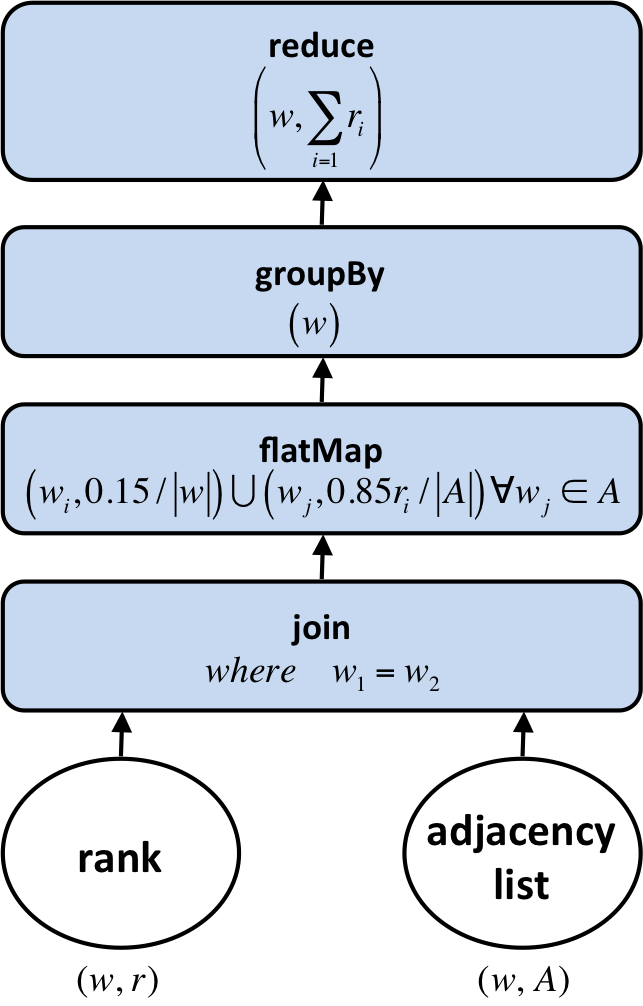
\includegraphics[width=.3\linewidth]{images/pageRankStep.png}
	\caption{Data flow of one iteration of the PageRank algorithm for Spark and Stratosphere.}
	\label{fig:pageRankDataFlow}
\end{figure}

For the comparison, we calculate $10$ steps of the PageRank algorithm for varying sizes of the adjacency matrix $A$.
The adjacency matrix $A$ is a sparse matrix of size $n \times n$ with a sparsity of $0.001$.
For each test run, the matrix is randomly generated so that their non-zero cell entries are uniformly distributed.
The computation is executed on $50$ cores of the DIMA cluster.
We set the block size to $500 \times 500$ and chose Breeze as math back end for Gilbert's distributed execution engines.
The runtimes are depicted in \cref{fig:pageRankResults}.

\begin{figure}
	\centering
	\begin{tikzpicture}
			\begin{loglogaxis}[
				xlabel={Number of vertices $n$},
				ylabel={Execution time $t$ in s},
				legend pos=north west,
				legend entries={Gilbert Spark, Gilbert Stratosphere, Specialized Stratosphere,Specialized Spark}
			]
			
			\addplot[blue,
				mark=x,
			] table[
				x=NumVertices,
				y=Time,
			]
			{data/pagerank/pagerankSpark};

			\addplot[red,
				mark=o,
			] table[
				x=NumVertices,
				y=Time,
			]
			{data/pagerank/pagerankStratosphere};

			\addplot[teal,
				mark=diamond,
			] table[
				x=rows,
				y=time,
			]
			{data/pagerank/pagerankBenchStratosphere};

			\addplot[black,
				mark=triangle,
			] table[
				x=rows,
				y=time,
			]
			{data/pagerank/pagerankBenchSpark};
			\end{loglogaxis}
		\end{tikzpicture}
	\caption{Execution time of $10$ steps of the PageRank algorithm on $50$-cores depending on the adjacency matrix's size.}
	\label{fig:pageRankResults}
\end{figure}

The graph shows that the directly implementend PageRank algorithm runs clearly faster than Gilbert's version of PageRank.
For Stratosphere, we were only able to compute Gilbert's PageRank for $50000$ websites, before the computation became too slow to execute.
Even though, the Spark execution engine showed a similar runtime behavior for $25000 \le n \le 50000$, Spark was able to scale up to $n=100000$.

The specialized algorithms show a better scalability.
For both systems, Spark and Stratosphere, we could compute the PageRank for up to $150000$ websites.
Interestingly, the Stratosphere system scales better for the specialized algorithm than Spark.
For $n\ge 25000$, Stratosphere shows significant faster runtimes.
It is not yet fully clear what causes this difference.
We assume that the fault tolerance mechanism of Spark is responsible for the performance loss.
With increasing number of iterations and data size, Spark also has to increase the lineage information stored for a possible data recovery.
This lineage information costs CPU time and consumes memory.
Since it is not possible to disable the fault-tolerance mechanism, one has to keep this aspect in mind when comparing Stratosphere with Spark.

The performance difference between the specialized algorithm and Gilbert's version can be explained by considering the different execution plans.
As shown in \cref{fig:pageRankDataFlow}, each iteration of the specialized PageRank algorithm comprises one join, one group reduce and one flat map operation.
The flat map operation can be executed without communication between the nodes.
The join and reduce operation requires the data to be sent over the network.
Thus, most of the time should be spent executing the join and reduce operation.

Looking at line 10 of \cref{lst:gilbertPageRank}, we see that we have to compute one matrix-vector product, two vector-scalar products and one vector sum for each iteration of Gilbert's PageRank algorithm.
Remembering \cref{sec:LinearAlgebraOperations}, we can deduce that all these operations require two cross, two join and one reduce operation.
The two cross operations, where one of the operands is a scalar value and thus only an one element data set, can be realized effciently by simply broadcasting the scalar value.
However, the two join operations and the reduce operation require to shuffle the available data and thus cause some serious network costs.

If we now compare the specialized algorithm with Gilbert's implementation, then we clearly see that the high-level linear algebra representation adds three additional operations, with one of them being highly expensive.
Therefore, it is not surprising that the specialized PageRank algorithm performs better.

\subsection{K-Means}

The k-means clustering algorithm~\cite{macqueen:1967a} is very popular for cluster analysis in data mining.
The goal of k-means is to partition the available $n$ data points into $k$ clusters, where each data point is assigned to the cluster with the nearest mean.
Even though to find the optimal solution is NP-hard, there exist heuristic algorithms.
The standard algorithm alternately assigns the data points to its nearest intermediate cluster and calculates new intermediate cluster center as the mean of all assigned data points.
The initial cluster centers are usually points randomly selected from the set of data points or random points.
The Matlab code for the k-means algorithm, shown in \cref{lst:kmeansMatlab} is a little bit cumbersome if one wants to write it down in matrix notation.

\begin{listing}[!h]
	\begin{CenteredBox}
		\begin{lstlisting}[language=Matlab]
		datapoints = load();
		centers = load();
		mask = repmat((1:numCenters), 1, numDatapoints);
		for i = 1:maxIterations
  			distances = pdist2(datapoints, centers); % pairwise distances
  			assignments = min(distances, [], 2); % index of nearest cluster center
  			repIdx = repmat(assignments', numCenters, 1);
  			multiplier = repIdx == mask; % indicator matrix
  			divisor = repmat(sum(multiplier,2),1, dimension);
  			centers = (multiplier*datapoints)./divisor;
		end
		\end{lstlisting}
	\end{CenteredBox}
	\caption{Matlab's k-means implementation.}
	\label{lst:kmeansMatlab}
\end{listing}

The data points and centers are stored rowwise in the matrices \code{data points} and \code{centers}.
The first step, assigning each data point to its nearest center, is done in the lines $5$ and $6$.
The \code{pdist2} function calculates the pairwise euclidean distance between the rows of its two operands, in our case the current centers and the data points.
Once we have all pairwise distances calculated, we can select for each data point its nearest cluster center.
This is done in line $6$.
The \code{assignments} column vector contains the index of the nearest cluster center for each data point.
In order to calculate the new cluster centers as the mean of all assigned data points, we have to introduce some repmat magic.
The idea is to construct for each center a logical row vector which indicates all data points assigned to this cluster.
We achieve this by generating a matrix which contains in each row the \code{assignments} vector.
The matrix has as many rows as there are clusters.
Then we compare this matrix in line $8$ with \code{mask} whose cells are set to the row index of the cell.
That gives us the aforementioned indicator matrix.
By adding the entries of each row, we know how many data points are assigned to the cluster centers.
The new cluster centers and thus the second step of the algorithm are obtained as the result of a matrix multiplication and cellwise matrix division in line $10$.	

Compared to the Matlab representation, the direct implementation for Spark and Stratosphere seems rather simple.
The first difference is that we represent the data points as tuples of the form $(id_i, p_i)$ with $id_i$ being an identifier of data point $i$ and $p_i$ being the coordinates of the data point.
The clusters are represented likewise as tuples $(id_j, c_j)$ with $c_j$ being the coordinates of the cluster center.
In order to calculate the pairwise distances between the data points $p_i$ and the clusters $c_j$ we first construct the cartesian product of the two datasets.
This gives us all combinations of data point cluster pairs.
Having the coordinates of the data point and the cluster center, we can easily compute the distance.
The output of the distance computation is again a tuple of the form $(id_i, p_i, id_j, \norm{p_i - c_j}_2)$, the data point id, the data point coordinates, the cluster center id and the distance.
By grouping on the data point id $id_i$ we can select the cluster center with the minimal distance.
The result of the reduce operation has the form $(id_j, p_i)$ with $id_j$ being the cluster center id.
In order to calculate the new cluster centers, we have to group on the cluster center id and add up all assigned data points $p_i$.
These operations constitute a single iteration step.
We obtain the k-means algorithm if we execute this plan repeatedly.
The dataflow plan is also depicted in \cref{fig:kmeansDataflow}.

\begin{figure}[h!]
	\centering
	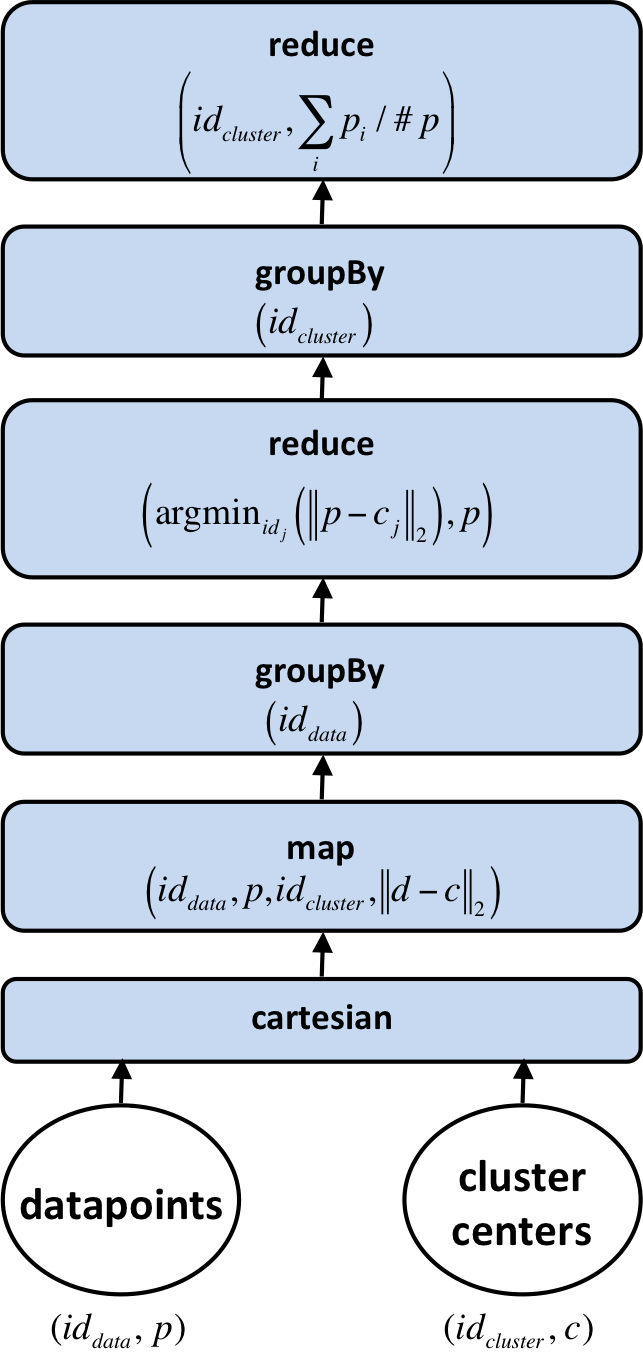
\includegraphics[width=0.3\linewidth]{images/kmeansStep.png}
	\caption{Dataflow plan of a single k-means step.}
	\label{fig:kmeansDataflow}
\end{figure}

We compare the runtime of Gilbert's k-means implementation with the runtime of the directly implemented algorithms.
The Gilbert code is given in \cref{lst:kmeansGilbert}.
As we can see, the only difference between Matlab's and Gilbert's version is the \code{fixpoint} and the \code{minWithIndex} function.
The \code{minWithIndex} function returns the minimum value of the specified dimension and its index as column vectors in a cell array.

\begin{listing}[!h]
	\begin{CenteredBox}
		\begin{lstlisting}[language=Matlab]
		datapoints = load();
		centers = load();
		mask = repmat((1:numCenters), 1, numDatapoints);
		function newCenters = kmeansStep(centers)
  			distances = pdist2(datapoints, centers);
		  	assignments = minWithIndex(distances, 2);
		  	repIdx = repmat(assignments{2}', numCenters, 1);
		  	multiplier = repIdx == mask;
		  	divisor = repmat(sum(multiplier,2),1, dimension);
		  	newCenters = (multiplier*datapoints)./divisor;
		end
		fixpoint(centers,@kmeansStep, maxIterations)
		\end{lstlisting}
	\end{CenteredBox}
	\caption{Gilbert's k-means implementation.}
	\label{lst:kmeansGilbert}
\end{listing}

For our experiments, we calculated $10$ steps of the k-means algorithms on the $50$ core DIMA cluster.
The algorithms computed $100$ cluster centers from $n$ data points.
The points were $2$-dimensional.
We varied the number of data points from $1000$ to $1000000$.
The data points and the initial cluster centers were drawn from a uniform distribution.
We set the block size to $500\times 500$.
The results of the experiment are depicted in \cref{fig:kmeansResult}.

\begin{figure}[h!]
	\centering
	\begin{tikzpicture}
			\begin{loglogaxis}[
				xlabel={Number of data points $n$},
				ymax=5000,
				ylabel={Execution time $t$ in s},
				legend pos=north west,
				legend entries={Gilbert Spark, Gilbert Stratosphere, Specialized Stratosphere}
			]
			
			\addplot[blue,
				mark=x,
			] table[
				x=NumDatapoints,
				y=Time,
			]
			{data/kmeans/kmeansSpark};

			\addplot[red,
				mark=o,
			] table[
				x=NumDatapoints,
				y=Time,
			]
			{data/kmeans/kmeansStratosphere};

			\addplot[teal,
				mark=diamond,
			] table[
				x=numDatapoints,
				y=time,
			]
			{data/kmeans/kmeansBenchStratosphere};
			\end{loglogaxis}
		\end{tikzpicture}
	\caption{Execution time of $10$ steps of the k-means algorithm on $50$-cores depending on the adjacency matrix's size.}
	\label{fig:kmeansResult}
\end{figure}

We observe that Gilbert's k-means implementations are slower than the specialized implementation.
For $n=100000$ the specialized implementation achieves a speed-up of $8$ and $10$ compared to the Spark executor and Stratosphere executor, respectively.
Additionally, we could only calculate $100000$ points with Gilbert, because for more points the computation took too long to finish.
Thus, we can conclude that the direct implementation of k-means executing on Stratosphere not only runs faster but also scales better.
Interestingly, we were not able to run the specialized algorithm on Spark because the two reduce operations caused too much work load.

If we take a closer look at the execution plans of both algorithms, it becomes clear why Gilbert performs so poorly.
For each step of the specialized algorithm, the dataflow system has to execute one cartesian, one map and two group reduce operations.
The two group reduce and the cartesian operation are responsible for most of the work load, because they cause significant network I/O.

For Gilbert, the execution plan is more complex.
Looking at the code in \cref{lst:kmeansGilbert} we have the following summation:
The \code{pdist2} function is implemented using one join, one map and one group reduce operation.
The \code{minWithIndex} function uses three cartesian, one group reduce and two cogroup operations.
The \code{repmat} function comprises three cartesian and one cogroup operation.
The comparison operator in line $8$ requires one join operation.
The matrix multiplication and cellwise matrix division in line $10$ is implemented using two join and one reduce operation.
In total, one step of Gilbert's k-means algorithm inflicts four join, nine cartesian, four cogroup and three group reduce operations.
Consequently, we can conclude that the linear algebra abstraction of Gilbert comes at the price of a more complex and thus longer running execution plan.

\section{Breeze vs. Mahout Math-Backend}

As we have explained in \cref{sec:mathBackend}, Gilbert supports two math back ends for the computation of local tasks.
The principal math back end uses the Breeze library for high performance linear algebra operations.
As an alternative, Gilbert also supports the popular Mahout math library.
In this section, we want to compare these two libraries against each other and assess which of them executes Gilbert programs faster.

As first benchmark, we repeated the matrix multiplication from \cref{subsec:mm} with the Mahout library.
The benchmark calculates the matrix multiplication of two sparse matrices $A,B\in\mathbb{R}^{n\times n}$ with $n$ being their dimensionality.
The matrices have a sparsity of $0.001$.
The computation is executed on $50$ cores and we use a block size of $500\times 500$.
The results are given in \cref{subfig:mmMathBackend}.

\begin{figure}
	\centering
	\begin{subfigure}{\dualpgfwidth}
		\begin{tikzpicture}
			\begin{semilogxaxis}[
				xlabel={Dimensionality $n$},
				ylabel={Execution time $t$ in s},
				legend pos=north west,
				legend entries={Breeze Spark, Breeze Stratosphere, Mahout Spark, Mahout Stratosphere},
				width=\dualpgfwidth,
			]
			
			\addplot[
				color=red,
				mark=o,
			] table[
				x=RowsA,
				y=Time,
			]
			{data/matrixMultLoad/matrixMultBreezeLoadSpark};
			
			\addplot[
				color=teal,
				mark=triangle,
			]table[
				x=RowsA,
				y=Time,
			]
			{data/matrixMultLoad/matrixMultBreezeLoadStratosphere};

			\addplot[
				color=blue,
				mark=x,
			] table[
				x=RowsA,
				y=Time,
			]
			{data/matrixMultLoad/matrixMultMahoutLoadSpark};

			\addplot[
				color=black,
				mark=diamond,
			]table[
				x=RowsA,
				y=Time,
			]
			{data/matrixMultLoad/matrixMultMahoutLoadStratosphere};
			
			\end{semilogxaxis}
		\end{tikzpicture}
		\caption{}
		\label{subfig:mmMathBackend}
	\end{subfigure}
	\begin{subfigure}{\dualpgfwidth}
		\begin{tikzpicture}
			\begin{semilogxaxis}[
				xlabel={Rows $d$ of $V$},
				ylabel={Execution time $t$ in s},
				legend pos=north west,
				legend entries={Breeze Spark, Breeze Stratosphere, Mahout Spark, Mahout Stratosphere},
				width=\dualpgfwidth,
			]
			
			\addplot[
				color=red,
				mark=o,
			] table[
				x=Rows,
				y=Time,
			]
			{data/nnmfStepLoad/nnmfStepBreezeLoadSpark};
			
			\addplot[
				color=teal,
				mark=triangle,
			]table[
				x=Rows,
				y=Time,
			]
			{data/nnmfStepLoad/nnmfStepBreezeLoadStratosphere};

			\addplot[
				color=blue,
				mark=x,
			] table[
				x=Rows,
				y=Time,
			]
			{data/nnmfStepLoad/nnmfStepMahoutLoadSpark};

			\addplot[
				color=black,
				mark=diamond,
			]table[
				x=Rows,
				y=Time,
			]
			{data/nnmfStepLoad/nnmfStepMahoutLoadStratosphere};
			
			\end{semilogxaxis}
		\end{tikzpicture}
		\caption{}
		\label{subfig:nmfMathBackend}
	\end{subfigure}
	\caption{Comparison of Breeze and Mahout math back end. \subref{subfig:mmMathBackend} Runtime of matrix multiplication on $50$-core cluster using Breeze and Mahout. \subref{subfig:nmfMathBackend} Runtime of single nnmf step on $50$-core cluster using Breeez and Mahout.}
	\label{fig:nnmfLoadMathBackend}
\end{figure}

The results of the matrix multiplication demonstrate impressively that Breeze is far superior to Mahout in multiplying two sparse matrices.
Even for relatively small matrix sizes of $n=2500$ the multiplication takes so long that it can hardly be regarded feasible.
Breeze reaches a speed-up of $100$ compared to Mahout.
The reason for this bad performance unveils a look into the code base of Mahout.
Mahout offers a sparse matrix implementation, based on hash maps.
However, it does not provide an efficient algorithm for this data structure.
Instead, Mahout uses the standard matrix multiplication algorithm derived from its definition.
Thus, for each resulting element $c_{i,j}$, Mahout iterates over the complete row $a_i$ of $A$ and column $b^{j}$ of $B$, even though most of the row and column entries will be zero.
Even worse, each access triggers an hash map look up.
In total, the matrix multiplication has to perform $2n^3$ hash table look ups and $n^3$ hash table insertions.

In contrast to Mahout, Breeze implements the sparse matrix using the compressed column sparse (CSC) storing scheme.
Not only does this avoid costly hash map look ups, because the data is stored in a continuous array, but Breeze also implements an optimized matrix multiplication algorithm.
The algorithm is aware of the sparse nature of its operands and accesses only elements which are non-zero in both matrices.

As second benchmark, we repeated the NMF computation from \cref{subsec:NMF}.
We calculated a single NMF step for varying number of rows $d$ of $V$ on $50$-cores of the cluster.
The number of rows $d$ reaches from $500$ to $10000$.
As before, the sparsity of $V$ is $0.001$ and its non-zero cells are distributed uniformly.
The sizes of $W$ and $H$ are $d\times 10$ and $10 \times 100000$, respectively.
For the benchmark, we set the block size to $500 \times 500$.
The runtimes of the Breeze and Mahout math back end are given in \cref{fig:nnmfLoadMathBackend}.

It can be clearly seen that NMF runs faster with Breeze as math back end on the Stratosphere as well as on the Spark execution engine.
On Spark, Breeze reaches a speed-up of roughly $4$ for $d=10000$. 
On Stratosphere, Breeze reaches a speed-up of about $1.75$ for the same number of rows.

We can conclude that Breeze has a better support for sparse matrix operations.
Its performance is also better for operations on mixed sparse and dense matrices as it is the case for NMF.
Therefore, we highly recommend using Breeze as the math back end in order to experience best performances with Gilbert programs.

